\subsection{Structure proposée pour la solution}

Au lieu de mapper l'audio erroné directement à l'audio corriger,
nous proposons un système qui enchaîne trois transformations.
La première transforme \(S_A\) en une représentation textuelle \(T_A\)
La deuxième produit un texte corrigé \(T_C\) à partir de \(T_A\).
La dernière étape est de produire \(S_C\) à partir de \(T_C\) (voir la Figure~\ref{fig.detail-system}).

\begin{figure}[hbt]
    \centering
    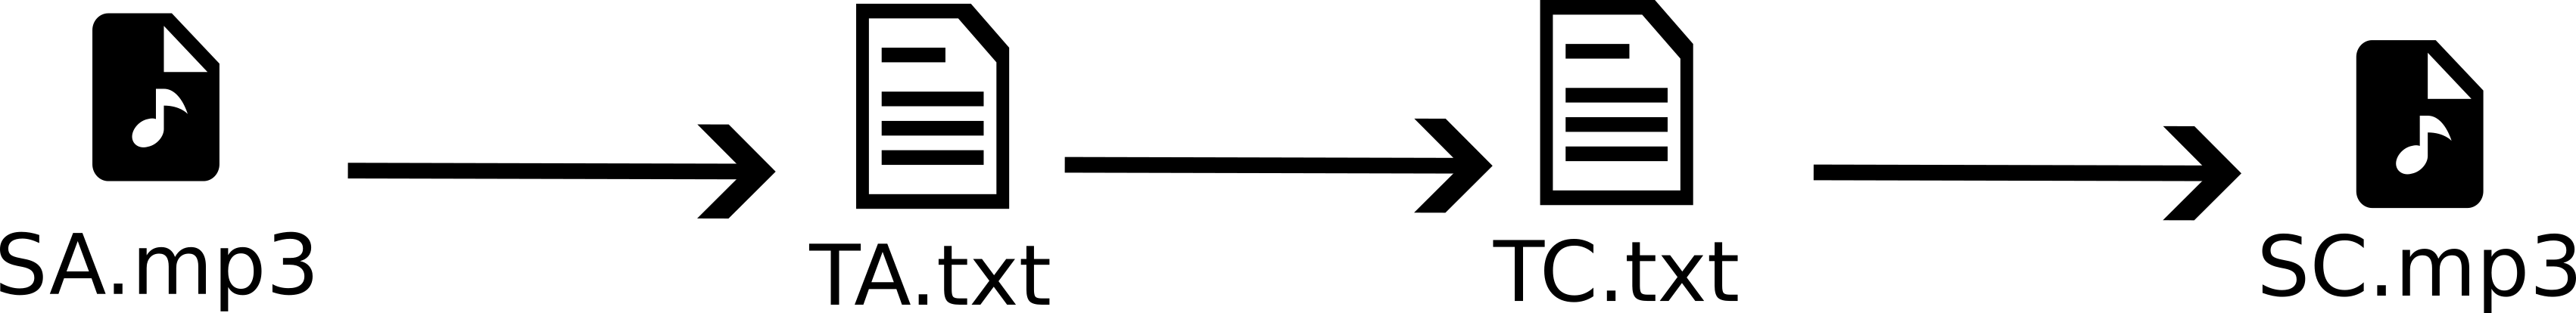
\includegraphics[width=\linewidth]{assets/images/detail.png}
    \caption{Étapes intermédiaires du système proposé.}
    \label{fig.detail-system}
\end{figure}

L'étape finale de cette procédure est la plus simple et peut être considérée comme résolue.
La tâche en question est tout simplement de produire un audio à partir d'un texte.
Il s'agit de synthèse vocale.
Plusieurs solutions existent pour cette tâche, y compris des solutions open-source~\cite{Tan_et_al._2022}.
Nous nous concentrerons donc sur les deux premières étapes.

La première partie de notre système réalise une transcription automatique de l'audio.
C'est une tâche de \gls{asr}, 
avec la complexité supplémentaire que la parole en question ne suit pas les lois usuelles du langage.
